\section*{Supplementary Material}
\Cref{sec:implementation,sec:properties} give the implementation and proofs. The remaining sections document the evaluations, ablations, and simulator rollouts.

\section{Implementation and evaluation details}
\label{sec:implementation}
\subsection{World-model architecture and training objective}
Model training and method evaluation use a server with eight RTX 5090 GPUs. The cost study in \cref{sec:cost} evaluates operation on a single RTX 3090.

The ResNet world models are pretrained offline on action--observation sequences; the \emph{Frozen} setting holds all pretrained weights fixed during test-time execution. For PushObj and PushT, the encoder uses a SmallResNetGeM visual backbone outputting a $d_v=384$-dimensional embedding, paired with a 6-layer action-conditioned Transformer predictor (16 attention heads, feed-forward width 2048, dropout 0.1). Proprioceptive states and 5-step action blocks are mapped through learned 10-dimensional linear embeddings ($d_p=10$). Each training window comprises four observations spaced five control steps apart, where three context frames predict the corresponding one-step-shifted targets. Action embeddings condition the Transformer predictor but are excluded from the reconstruction target.

Let $z_i^o=[z_i^v;z_i^p]\in\R^{d_o}$ denote the concatenated observation latent of total dimension $d_o=d_v+d_p$, let $\hat z_{i+1}^o$ denote the teacher-forced one-step prediction, and let $\operatorname{sg}(\cdot)$ denote the stop-gradient operator. The offline training loss combines mean-squared latent prediction with the Temporal Straightening (TS) training objective~\cite{wang2026straightening}:
\begin{align}
 \mathcal L_{\rm WM}&=\frac{1}{3d_o}\sum_{i=0}^{2}
 \norm{\hat z_{i+1}^o-\operatorname{sg}(z_{i+1}^o)}^2
 +\lambda_{\rm TS}\mathcal L_{\rm TS},\\
 \mathcal L_{\rm TS}&=\operatorname{mean}_{i\in\mathcal V}
 \left[1-\frac{\langle\Delta z_i^v,\Delta z_{i+1}^v\rangle}
 {\norm{\Delta z_i^v}\norm{\Delta z_{i+1}^v}}\right],
\end{align}
where $\Delta z_i^v=z_{i+1}^v-z_i^v$ and $\lambda_{\rm TS}$ weights the straightening regularizer. The set $\mathcal V$ comprises valid adjacent displacement pairs across the training batch whose Euclidean norms both exceed $10^{-6}$ (using the same numerical floor in the cosine denominator, and setting $\mathcal L_{\rm TS}=0$ if $\mathcal V=\emptyset$). Note that $\mathcal L_{\rm TS}$ acts on observed visual embeddings, whereas the prediction loss averages uniformly across all $d_o$ coordinates (in contrast to the branch-normalized planning metric in \cref{eq:metric}). Target representations are detached via stop-gradient rather than an exponential moving average (EMA).

For our augmented-data PushObj checkpoints, we train for 3 epochs with $\lambda_{\rm TS}=0.01$, effective batch size 64, and bf16 mixed precision over 1,630,266 training windows and 403,951 validation windows. The visual encoder is optimized using Adam ($\text{lr}=10^{-5}$), while the predictor and action/proprioceptive embedders use AdamW ($\text{lr}=5\times10^{-4}$, weight decay $0.01$), both with $(\beta_1,\beta_2)=(0.9,0.999)$ and constant learning rates. The headline checkpoint additionally trains a detached pixel decoder in the last epoch. Planning uses the same encoder and predictor.

For Maze, we directly evaluate the published SmallResNet checkpoint (without GeM pooling, trained with $\lambda_{\rm TS}=0.001$ and identical Transformer dimensions) without any new offline training. Both released checkpoints correspond to epoch~3 snapshots from a configured 5-epoch schedule.

\subsection{Interaction-biased data collection}
We collect training and validation trajectories for each seen shape using the contact bias and Gaussian noise in \cref{tab:parameters}. Source placements use up to four retries, position jitter of 20 pixels, and orientation jitter of 0.3 radians. The simulator receives pixel displacements divided by 100. We retain valid trajectories with physical contact and displacements under 80 pixels per action block. Training and validation use disjoint source pools. The overlap between the released model's pretraining data and evaluated targets is undocumented.

\subsection{Receding-horizon planning and online adaptation}
MPC optimizes a 25-control horizon and executes the first five controls. Adam runs 100 iterations per replan with a cosine schedule from 0.1 to zero. Planning starts from zero displacements, then warm-starts by shifting the unexecuted suffix and padding with zeros. The optimizer adds no action noise.

AdaJEPA updates after each executed block using the five most recent transition segments and one-step prediction loss without straightening. It updates the last Transformer block, final normalization layer, and encoder output projection. Learning rates are $5\times10^{-4}$ for the predictor and $10^{-5}$ for the encoder. Each update starts a fresh Adam optimizer and enables dropout only during adaptation. Each episode starts from the offline checkpoint.

\subsection{Task success}
PushObj and PushT require both the joint pusher--object position error and the wrapped orientation error to fall below the tolerances in \cref{tab:parameters} at a replan boundary. Maze uses the goal-distance tolerance. Runs stop on success, with per-control stopping for the medium-route protocol in \cref{tab:maze-medium-threshold}.

\subsection{Planner objectives and execution order}
\label{sec:parameters}
Each planning call encodes its observations and stored memories once with the current encoder.

\begin{table*}[t]
\centering
\caption{\textbf{ECP settings for ResNet control.} Parameters apply to PushObj, PushT, and Maze; each replan executes five controls. Loss-gate settings apply to AdaJEPA~\cite{wang2026adajepa}. Setting $\kappa=0$ or $b=1$ disables memory or goal reweighting, respectively.}
\label{tab:parameters}
\small
\begin{tabular}{p{0.15\textwidth}p{0.53\textwidth}p{0.23\textwidth}}
\toprule
Symbol & Meaning & Value or domain\\
\midrule
$d_v,d_p$ & Flattened visual and proprioceptive branch dimensions & 384, 10\\
$A=(a_1,\ldots,a_H)$ & Candidate sequence; each $a_h$ contains five control calls & 25 control calls total\\
$H,\hat z_{t,h}$ & Predicted latent horizon and its $h$-th state & $H=5$\\
$W,r_t,w_t$ & Motion window, normalized displacement, and trigger weight & $W=3$; $w_t\in[0,1]$\\
$\gamma_{\rm lo},\gamma_{\rm hi}$ & Full-weight and zero-weight motion thresholds & 0.15, 0.45 (main PushObj); 0.05, 0.15 (PushT, Maze, component studies)\\
$\epsilon$ & Numerical floor for squared distances and loss ratios & $10^{-12}$\\
$\beta,\kappa$ & Squared-radius fraction and regularizer strength & 0.25, 2\\
$\alpha_t,b$ & Current proprioceptive weight and trigger multiplier & $\alpha_t\in\{1,10\}$; $b=10$\\
$W_g,\tau_g$ & Separation of loss windows and relative-improvement threshold & 3 replans, 0.05\\
$b_c,\sigma_c,\eta_i$ & Collection bias, per-axis noise scale, and standard Gaussian noise & 9 px, 10 px, $\mathcal N(0,I_2)$\\
$a_{\max},n_{\rm exec}$ & Action-offset magnitude cap and number of executed controls & 15 px, 5 calls\\
Training trajectories & Interaction-biased PushObj per seen shape & 4,000 train, 1,000 validation\\
Success tolerances & Joint position and wrapped orientation errors (PushObj/PushT), goal distance (Maze) & 20 px and $\pi/9$, 0.5 units\\
\bottomrule
\end{tabular}
\end{table*}

\paragraph{Native objectives.}
PushObj uses terminal goal distance for its first five replans and switches to the all-frame objective below. Maze uses the all-frame objective throughout. The current observation is included as step zero.
\begin{equation}
J_{\rm all}(A;\alpha)=
\frac{\sum_{h=0}^{H}2^h D_\alpha(\hat z_{t,h}(A),z_g)}
     {(H+1)\sum_{h=0}^{H}2^h}.
\label{eq:baseexact}
\end{equation}
Memory uses the same outer horizon normalization over predicted states.

\paragraph{Feedback order.}
The controller measures prediction loss, updates AdaJEPA when enabled, then detects stalls with the updated encoder. A detected stall stores the current observation. With first-stall activation, the memory and task-specific correction take effect at the next plan. The loss gate in \cref{eq:gate} releases stored memories once the loss plateaus at a stall. Subsequent stalls renew the temporary reweighting, and stored memories last for the episode. Warm-up is ten replans on PushObj and four in the main Maze gating study.

\subsection{Paired evaluation and statistical testing}
\label{sec:paired}
On PushObj, PushT, and Maze, paired runs share task instances. The objectives coincide until intervention, and the audit checks that actions and states match over this prefix. We reuse non-triggered trajectories and rerun all tasks for permanent reweighting. The exact two-sided McNemar test compares discordant successes. Rescue and harm count tasks that switch from failure to success and from success to failure, respectively.

\begin{table*}[t]
\centering
\caption{\textbf{PushT results by checkpoint and visual shift.} Ours combines the interaction-biased checkpoint (Data aug.) with ECP on. Released uses the published ResNet checkpoint. Success (\%) is measured on 50 matched tasks per condition over 30 replans of five controls. Frozen fixes weights, and AdaJEPA updates them online. S\&P is salt-and-pepper noise. Avg. excludes Clean.}
\label{tab:pusht-ecp}
\small
\setlength{\tabcolsep}{3.7pt}
\begin{tabular*}{\textwidth}{@{\extracolsep{\fill}}llcrrrrrrrr@{}}
\toprule
Checkpoint & Updates & ECP & Clean & Blur & S\&P & Dark & Red agent & Red object & Red goal & Avg.\\
\midrule
Released & Frozen & Off & 60 & 50 & 60 & 52 & 56 & 10 & 36 & 44.0\\
Released & Frozen & On & 68 & 56 & 60 & 58 & 56 & 10 & 38 & 46.3\\
Released & AdaJEPA & Off & 82 & 76 & 76 & 76 & 60 & 10 & 40 & 56.3\\
Released & AdaJEPA & On & 84 & 80 & 78 & 80 & 62 & 10 & 40 & 58.3\\
\midrule
Data aug. & Frozen & Off & 72 & 58 & 62 & 70 & 56 & 12 & 18 & 46.0\\
Data aug. & Frozen & \textbf{On} & 82 & 72 & 70 & 78 & 68 & 12 & 34 & \textbf{55.7}\\
Data aug. & AdaJEPA & Off & 86 & 82 & 80 & 86 & 64 & 16 & 42 & 61.7\\
Data aug. & AdaJEPA & \textbf{On} & 86 & 86 & 80 & 88 & 68 & 18 & 42 & \textbf{63.7}\\
\bottomrule
\end{tabular*}
\end{table*}


\section{Mathematical properties of the stagnation regularizer}
\label{sec:properties}
We now formalize the two structural properties of the stagnation regularizer $\mathcal R_t^{\rm stall}$ stated in \cref{sec:memory}. Write the branch-normalized metric in quadratic form as $D_{\alpha_0}(z,m)=(z-m)^\top Q(z-m)$, where, for the base weight $\alpha_0>0$, the positive-definite diagonal metric tensor is
\begin{equation}
 Q=\operatorname{diag}\!\left(d_v^{-1}I_{d_v},\,
 \alpha_0d_p^{-1}I_{d_p}\right).
\end{equation}
For any memory anchor $m_j$ at positive distance $d_g=D_{\alpha_0}(m_j,z_g)>0$ from the goal such that $\beta d_g\geq\epsilon$, the squared support radius is $\rho_j=\beta d_g$. Evaluating the kernel $K_j(z)$ of \cref{eq:kernel} at the goal $z=z_g$ yields:
\begin{equation}
 K_j(z_g)=\left[1-\frac{d_g}{\beta d_g}\right]_+^2=[1-1/\beta]_+^2=0\quad(0<\beta<1).
\end{equation}
Geometrically, in the norm induced by $Q$, the kernel's support is an open ball of radius $\sqrt{\beta d_g}$ centered at $m_j$, whose boundary remains at a strictly positive margin $(1-\sqrt{\beta})\sqrt{d_g}>0$ away from $z_g$. Thus every active memory kernel strictly excludes the goal from its support.

For any predicted state $z$ strictly inside the support ($D_{\alpha_0}(z,m_j)<\rho_j$), the derivative of \cref{eq:kernel} with respect to the predicted latent state is:
\begin{equation}
 \nabla_zK_j(z)=-\frac{4}{\rho_j}
 \left(1-\frac{D_{\alpha_0}(z,m_j)}{\rho_j}\right)Q(z-m_j).
 \label{eq:kernelgradient}
\end{equation}
During gradient-based action optimization (which minimizes \cref{eq:objective}), the negative gradient $-\nabla_z K_j(z)$ points away from the anchor along $Q(z-m_j)$, repelling the predicted rollout state away from the stalled anchor $m_j$. As $D_{\alpha_0}(z,m_j)\uparrow\rho_j$, both $K_j(z)\to 0$ and $\nabla_z K_j(z)\to 0$, guaranteeing $C^1$ smoothness across the support boundary and zero gradient perturbation outside the kernel support. (At the anchor $z=m_j$, the kernel reaches its maximum, $K_j(m_j)=1$, with zero gradient $\nabla_z K_j(m_j)=0$.)

Propagating this state gradient back to the candidate action sequence $A$ via the predictor's action-to-latent Jacobian $G_{t,h}=\partial\hat z_{t,h}(A)/\partial A$ yields the total regularizer gradient:
\begin{equation}
 \nabla_A\mathcal R_t^{\rm stall}(A)=
 \sum_{h=1}^{H}\pi_h G_{t,h}^{\top}
 \sum_{j\in\mathcal M_t}w_js_j\nabla_zK_j(\hat z_{t,h}(A)).
\end{equation}
The world-model Jacobian maps the latent repulsion to action gradients. Repeated stalls can add penalties in the same neighborhood.

The $\epsilon=10^{-12}$ floor keeps degenerate denominators finite. When it is active, exact goal exclusion need not hold, while the full-latent memory amplitude $s_j$ also vanishes with its goal distance. An explored proprioceptive-space variant replaces only the kernel distance and radius with $\norm{z^p-m^p}^2/d_p$ and $\max\{\beta\norm{m^p-z_g^p}^2/d_p,\epsilon\}$; it retains the full-latent amplitude. All main $S$ results use the full-latent version.

\section{Benchmark comparison protocols}
\label{sec:benchmark}
\subsection{PushObj protocol}
\label{sec:pushobj-comparison}
\Cref{tab:main} uses the archived PushObj task list for DINO-WM and LeWM and a second list with the same shapes for ResNet models. For each backbone, Native and ECP share tasks and planning budgets. GD and CEM use the same horizon, execution block, and objective schedule. GD uses the settings in \cref{sec:implementation}. CEM uses 200 candidates, 30 elites, and ten iterations per replan.

\subsection{PushT and visual distribution shifts}
\label{sec:pusht-extension}
The PushT benchmark evaluates a common, fixed list of 50 start--goal pairs across clean observations and six visual distribution shifts: Gaussian blur ($\sigma=2$), salt-and-pepper impulse noise (1\% salt, 1\% pepper), darkened lighting (intensity scale $0.9$), and RGB recoloring (to red) of the pusher agent, manipulated T-block, or background goal anchor. The ResNet ECP configuration is transferred from PushObj ($\gamma_{\rm hi}=0.15$) without tuning.

\paragraph{Controller configurations.}
All PushT methods share the same tasks and control budget. DINO-WM uses its three-epoch T16k checkpoint and replans every 25 controls with a terminal goal cost. LeWM GD and the ResNet controllers replan every five controls. DINO-WM uses 100 steps in GD or 300 candidates, 30 elites, and 30 iterations in CEM. LeWM CEM and DDP-WM CEM use the PushObj CEM settings. The matched pairs in \cref{tab:pusht-ecp} agree up to the first intervention.

The checkpoint matrix in \cref{tab:pusht-ecp} separates the contribution of data, adaptation, and ECP. Within each block, toggling ECP keeps the checkpoint and update rule fixed; success is preserved or improved across all clean and shifted conditions. Comparing training recipes then shows how interaction-biased data and online correction work together.

The shifts also probe different parts of the visual task. Agent recoloring changes the controlled effector, object recoloring changes the manipulated body, and goal recoloring changes the target cue. Keeping the start--goal pairs fixed makes these conditions directly comparable. The common stopping rule evaluates physical alignment, so improvement reflects completed interactions under the altered observations.

% Keep supplementary figure pages aligned to the same top margin as text pages.
\makeatletter
\setlength{\@fptop}{0pt}
\setlength{\@dblfptop}{0pt}
\makeatother
\clearpage
\begin{table*}[!t]
\par\smallskip
\noindent \begin{minipage}[t]{\columnwidth}
\vspace{0pt}
\Cref{tab:extra-baselines} tests whether fixed visual representations alone account for robustness on the shifted PushT tasks. R3M~\cite{nair2022r3m}, DINOv2 CLS~\cite{oquab2024dinov2}, and DDP-WM~\cite{yin2026ddpwm} share the same CEM budget and task list.\par\smallskip
\normalsize
These controls change the visual representation while keeping the planning budget fixed. Both ECP controllers in \cref{tab:main} achieve higher mean success, supporting the role of execution feedback alongside representation learning.\par
\end{minipage}\hfill
\begin{minipage}[t]{\columnwidth}
\vspace{0pt}
\par\smallskip
{\centering
\centering
\captionof{table}{\textbf{Representation baselines on shifted PushT.} Success (\%) on 50 matched tasks per condition, with fixed weights, CEM, and 150 controls. S\&P denotes salt-and-pepper noise; Agent/Object/Goal recolor that component red. Avg. is the mean over six shifts, excluding clean observations.}
\label{tab:extra-baselines}
\small\setlength{\tabcolsep}{2pt}
\begin{tabular}{lrrrrrrr}
\toprule
Method & Blur & S\&P & Dark & Agent & Object & Goal & Avg.\\
\midrule
R3M &30&16&2&32&32&18&21.7\\
DINO CLS &30&16&56&42&22&42&34.7\\
DDP-WM &56&22&66&62&42&68&52.7\\
\bottomrule
\end{tabular}

\par}
\end{minipage}\par
\par\smallskip
\noindent \begin{minipage}[t]{\columnwidth}
\vspace{0pt}
\section{Cross-backbone transfer studies}
\label{sec:backbone}
\subsection{Transfer to LeWorldModel (LeWM)}
We train matched random-action and interaction-biased LeWM models~\cite{maes2026lewm} with the same data volume and schedule. This comparison separates learning from more useful interactions from correcting a stall at test time.\par\smallskip
\normalsize
For LeWM, ECP guides the pusher toward a contact waypoint after a stall. This tests whether a correction tied to the unfinished physical interaction can turn latent planning into object motion. The waypoint uses the observed object pose and geometry:
\[
 J_{\rm contact}(A)=10\operatorname{mean}_{k=1,\ldots,5;\,d=x,y}
 \left(\frac{\hat p_{k,d}(A)-q_d}{\sigma_{p,d}}\right)^2.
\]
Here $q$ is the waypoint and $\sigma_p$ scales each position coordinate by its dataset standard deviation. The five predicted pusher positions follow differentiable PD dynamics. Guidance lasts four replans per trigger, with at most seven guided replans per episode.

\Cref{tab:lewm-contact} holds model weights fixed during evaluation. Interaction-biased training improves native planning, and triggered contact guidance adds a further gain under both data recipes. Thus the training data and the execution-conditioned objective contribute at different stages of the controller.\par
\end{minipage}\hfill
\begin{minipage}[t]{\columnwidth}
\vspace{0pt}
\par\smallskip
{\centering
\centering
\captionof{table}{\textbf{LeWM data and planner ablations on PushObj.} All rows evaluate 350 tasks with fixed weights and a 150-control budget. Both data recipes use 16k training and 4k validation trajectories for ten epochs. The contact variant uses a 50-control warm-up and stall thresholds 0.15/0.45 (low/high).}
\label{tab:lewm-contact}
\small
\begin{tabular}{lrr}
\toprule
Planner & Success / 350 & Rate (\%)\\
\midrule
\multicolumn{3}{l}{Random actions}\\
Native &166&47.4\\
ECP contact guidance &186&53.1\\
\midrule
\multicolumn{3}{l}{Interaction-biased actions}\\
Native &215&61.4\\
Stagnation regularizer &216&61.7\\
Regularizer + pusher weighting &217&62.0\\
Intermittent contact offset &215&61.4\\
Four-replan offset, cap 15 px &218&62.3\\
Four-replan offset, 3--20 px &217&62.0\\
Contact weight 20 &227&64.9\\
\textbf{Contact weight 10 (ours)} &231&\textbf{66.0}\\
\bottomrule
\end{tabular}
\par}
\par\smallskip
\normalsize
The contact audit checks how that gain arises. Among 134 stalled tasks, guidance increases contact within 15 controls from 46 to 82 tasks, while cases reducing object error by more than five pixels increase from 11 to 34. Tracking both outcomes connects the correction to useful object motion. The offset controls test a prescribed displacement; the strongest result comes from optimizing contact guidance within planning. This lets the controller select actions under the world model while execution determines when to intervene.\par
\end{minipage}\par
\par\smallskip
\noindent \begin{minipage}[t]{\columnwidth}
\vspace{0pt}
\subsection{Transfer of interaction-biased data to DINO-WM}
\label{sec:dinowm}
\Cref{tab:dinowm-aug} changes the training actions while holding the DINO-WM architecture, training schedule, and CEM planner fixed. The tested variable is the interaction data.\par\smallskip
\normalsize
Augmentation improves every evaluated shape, showing that the data benefit transfers beyond the ResNet controller. This comparison uses native planning with six replans of 25 controls, isolating the offline data contribution from ECP intervention.\par
\end{minipage}\hfill
\begin{minipage}[t]{\columnwidth}
\vspace{0pt}
\par\smallskip
{\centering
\centering
\captionof{table}{\textbf{Augmentation improves DINO-WM on every shape.} PushObj success (\%) on 50 tasks per shape, with fixed weights, CEM, and 150 controls. Both models train for three epochs, differing only in action data. Sq./sT mean square/small-T; Avg. is mean success across all seven evaluated shapes.}
\label{tab:dinowm-aug}
\small
\setlength{\tabcolsep}{3.4pt}
\begin{tabular}{lrrrrrrrr}
\toprule
Training data & I & L & Sq. & Z & sT & $+$ & T & Avg.\\
\midrule
Ordinary actions &8&42&4&20&24&34&40&24.6\\
\textbf{Augmented (ours)} &16&72&14&46&56&66&72&\textbf{48.9}\\
\bottomrule
\end{tabular}
\par}
\end{minipage}\par

\end{table*}
\clearpage
\begin{table*}[!t]
\par\smallskip
\noindent \begin{minipage}[t]{\columnwidth}
\vspace{0pt}
Representation controls use R3M~\cite{nair2022r3m}, DINOv2~\cite{oquab2024dinov2}, and DDP-WM~\cite{yin2026ddpwm} with a shared budget (\cref{tab:extra-baselines}).
\end{minipage}\hfill
\begin{minipage}[t]{\columnwidth}
\vspace{0pt}
These controls separate representation, data, and planning gains. We next examine detection and memory.
\end{minipage}\par
\par\smallskip
\noindent \begin{minipage}[t]{\columnwidth}
\vspace{0pt}
\section{Extended trigger-threshold analysis}
\label{sec:threshold-details}
This sweep tests robustness to detection sensitivity. The checkpoint, tasks, and planner stay fixed while the high threshold varies over a fourfold range.\par\smallskip
\normalsize
Larger thresholds detect stalls earlier and in more episodes. Success remains above native planning throughout the sweep, while the rescue/harm counts show that the gain comes from recovering stalled tasks with few regressions. \Cref{tab:threshold-shape} locates this effect by shape: frozen ECP improves both seen and unseen groups, and AdaJEPA gains concentrate on seen shapes.\par
\end{minipage}\hfill
\begin{minipage}[t]{\columnwidth}
\vspace{0pt}
\par\smallskip
{\centering
\centering
\captionof{table}{\textbf{PushObj stall-threshold sweep.} ECP uses memory and goal reweighting with an augmented-data ResNet and AdaJEPA. All rows use 350 tasks and 30 replans. The low threshold is $\gamma_{\rm lo}=\gamma_{\rm hi}/3$. Triggered counts episodes with a stall, and First gives their median first-trigger replan.}
\label{tab:threshold}
\small
\setlength{\tabcolsep}{4pt}
\begin{tabular}{lrrrr}
\toprule
$\gamma_{\rm hi}$ & Success (\%) & Triggered & First & Rescue / harm\\
\midrule
Native &74.9&---&---&---\\
0.15 &76.9&90&14&8 / 1\\
0.30 &77.4&101&12&11 / 2\\
0.45 &77.7&108&11&11 / 1\\
0.60 &77.4&111&10&11 / 2\\
\bottomrule
\end{tabular}
\par}
\end{minipage}\par
\par\smallskip
{\centering
\captionof{table}{\textbf{PushObj threshold sweep by shape.} Success (\%) on 50 tasks per shape over 30 replans. Frozen fixes an augmented-data ResNet, and AdaJEPA updates it online. ECP uses memory and goal reweighting. Seen averages L, Z, $+$, T. Unseen averages I, square (Sq.), small-T (sT).}
\label{tab:threshold-shape}
\small
\begin{tabular*}{\textwidth}{@{\extracolsep{\fill}}ll*{10}{r}@{}}
\toprule
Updates & Planner / $\gamma_{\rm hi}$ & I & L & Sq. & Z & sT & $+$ & T & Seen & Unseen & All\\
\midrule
Frozen & Native & 32 & 72 & 42 & 72 & 58 & 74 & 78 & 74.0 & 44.0 & 61.1\\
 & ECP 0.45 & 46 & 84 & 46 & 92 & 62 & 88 & 88 & 88.0 & 51.3 & 72.3\\
\midrule
AdaJEPA & Native & 52 & 88 & 50 & 94 & 72 & 84 & 84 & 87.5 & 58.0 & 74.9\\
 & ECP 0.15 & 56 & 90 & 50 & 96 & 72 & 86 & 88 & 90.0 & 59.3 & 76.9\\
 & ECP 0.30 & 56 & 92 & 52 & 96 & 70 & 86 & 90 & 91.0 & 59.3 & 77.4\\
 & ECP 0.45 & 54 & 92 & 50 & 98 & 72 & 88 & 90 & 92.0 & 58.7 & 77.7\\
 & ECP 0.60 & 54 & 92 & 50 & 100 & 70 & 86 & 90 & 92.0 & 58.0 & 77.4\\
\bottomrule
\end{tabular*}
\par}
\par\smallskip
\noindent \begin{minipage}[t]{\columnwidth}
\vspace{0pt}
\section{Additional PushObj ablations and controls}
\label{sec:additional-controls}
\subsection{Memory and planning controls}
\Cref{tab:memory-strength} tests what a memory should represent. Joint visual--proprioceptive memory can distinguish scenes with the same pusher position but different object configurations. It improves success over proprioception-only memory at each tested strength.\par\smallskip
\normalsize
The search controls (\cref{tab:timing}) use eight two-step prefixes or a ten-step triggered continuation, with three interventions separated by four replans. ECP alone recovers the most tasks while preserving native successes.\par
\end{minipage}\hfill
\begin{minipage}[t]{\columnwidth}
\vspace{0pt}
\par\smallskip
{\centering
\centering
\captionof{table}{\textbf{Joint latent memory outperforms proprioception-only memory.} PushObj success (\%) on 350 tasks with 30 replans and an augmented-data ResNet updated by AdaJEPA. $\kappa$ scales the memory penalty; Joint combines visual and proprioceptive distances. Goal reweighting is disabled; native success is 74.9\%.}
\label{tab:memory-strength}
\small
\begin{tabular}{lrrr}
\toprule
Memory distance & $\kappa=0.5$ & $\kappa=2$ & $\kappa=8$\\
\midrule
Proprioceptive &75.1&74.9&75.1\\
Joint latent &75.4&76.0&75.7\\
\bottomrule
\end{tabular}
\par}
\end{minipage}\par
\par\smallskip
\noindent \begin{minipage}[t]{\columnwidth}
\vspace{0pt}
\subsection{Evaluation and training variability}
\label{sec:eval-seeds}\label{sec:replication}
\par\smallskip
{\centering\captionof{table}{\textbf{PushObj sensitivity to evaluation randomness.} Success (mean \% $\pm$ sample SD) on the same 350 tasks across three evaluation seeds. Aug. denotes interaction-biased training.}
\label{tab:eval-seeds}
\small
\begin{tabular*}{\columnwidth}{@{\extracolsep{\fill}}llr@{}}
\toprule
Controller & Training / planning & Success (\%)\\
\midrule
Frozen (ResNet) & Aug. + ECP (ours) & $72.29\pm0.00$\\
LeWM & Aug. + ECP (ours) & $66.00\pm0.00$\\
\midrule
AdaJEPA & Base data & $68.76\pm1.41$\\
AdaJEPA & Augmented data & $73.90\pm1.19$\\
AdaJEPA & \textbf{Aug. + ECP (ours)} & \textbf{76.86}$\pm1.03$\\
\bottomrule
\end{tabular*}
\par}
\end{minipage}\hfill
\begin{minipage}[t]{\columnwidth}
\vspace{0pt}
\par\smallskip
{\centering
\captionof{table}{\textbf{Training-seed variability on PushObj.} Native success (mean \% $\pm$ sample SD) across three augmented-data ResNet checkpoints. Frozen fixes weights, and AdaJEPA updates them online.}
\label{tab:training}
\small
\begin{tabular}{lrr}
\toprule
Targets / budget & Frozen & AdaJEPA\\
\midrule
350 tasks / 20 replans &$58.57\pm2.16$&$70.19\pm2.33$\\
700 tasks / 30 replans &$57.90\pm3.45$&$71.19\pm2.44$\\
\bottomrule
\end{tabular}
\par}
\par\smallskip
Evaluation seeds and training checkpoints test distinct sources of variability. Frozen and LeWM are deterministic; AdaJEPA varies through dropout, with both gains preserved. A disjoint 280-task stream also improves with either activation rule, especially first-stall activation.\par

\end{minipage}\par

\end{table*}
\clearpage
\begin{table*}[!t]
\par
\noindent \begin{minipage}[t]{\columnwidth}
\vspace{0pt}
\subsection{Post-trigger recovery and action-space correction}
\label{sec:behavior}\label{sec:action-space}
After the shared prefix, ECP increases pusher displacement and object progress. \Cref{fig:push-distance} shows completion from the same frozen checkpoint.\par\smallskip
{\centering
\captionof{table}{\textbf{Physical action correction on PushObj.} Success (\%) with AdaJEPA on 350 tasks per stream, 30 replans. Streams share 35 target segments and 41 source episodes.}
\label{tab:action}
\small
\begin{tabular}{lrrr}
\toprule
Task stream & Native & Action offset & Rescue / harm\\
\midrule
Stream A &74.9&77.4&10 / 1\\
Stream B &74.3&78.9&16 / 0\\
\bottomrule
\end{tabular}
\par}
\par\smallskip
After ten warm-up replans, movement below 10 pixels over three replans triggers five offsets: one fifth of the remaining displacement, capped at 15 pixels, with three-replan goal reweighting. Up to seven interventions are spaced four replans apart. Both streams improve.\par

\end{minipage}\hfill
\begin{minipage}[t]{\columnwidth}
\vspace{0pt}
\par\smallskip
{\centering
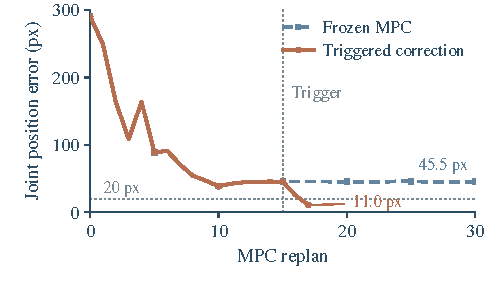
\includegraphics[width=\columnwidth]{figures/figS_pushobj_distance.pdf}
\captionof{figure}{\textbf{ECP completes a stalled PushObj episode.} Both runs use the same fixed, pretrained ResNet. Dashed/solid curves show native/ECP joint pusher--object position error in pixels. Vertical/horizontal lines mark stall detection and the 20-pixel success threshold. Only ECP crosses the threshold, at replan 17, with object-angle error also below $\pi/9$.}
\label{fig:push-distance}
\par}

\end{minipage}\par
\par
\noindent \begin{minipage}[t]{\columnwidth}
\vspace{0pt}
\section{Computational cost}
\label{sec:cost}
To test feasibility with lower compute, each planning run uses a single RTX 3090. Native and ECP share a fixed checkpoint and tasks; paired ten-task batches run sequentially on the same GPU with alternating order. The implementation uses PyTorch 2.3.0 and CUDA 12.1.\par\smallskip
\normalsize
GPU-synchronized timers include CUDA Graph capture and simulator replay, excluding model loading and the separate physics audit. \Cref{tab:cost} shows that fewer replans offset the per-replan overhead and reduce mean task time. Peak allocated memory stays below one GiB.\par

\end{minipage}\hfill
\begin{minipage}[t]{\columnwidth}
\vspace{0pt}
\par\smallskip
{\centering
\centering
\captionof{table}{\textbf{Planning time and memory on PushObj.} 350 paired tasks, fixed ResNet. Task time includes failures capped at 30 replans. P95: 95th percentile; memory: maximum PyTorch peak.}
\label{tab:cost}
\small
\setlength{\tabcolsep}{3.5pt}
\begin{tabular*}{\columnwidth}{@{\extracolsep{\fill}}lrr@{}}
\toprule
Metric & Without ECP & With ECP\\
\midrule
Success (\%) &61.14&72.29\\
Mean replans / task &15.59&13.66\\
Planning (ms / replan) &747.24&768.27\\
GD (ms / replan) &747.14&752.39\\
Mean task time (s) &15.25&13.41\\
P95 task time (s) &31.60&32.49\\
Total planning time (s) &4078.45&3672.32\\
Peak allocated memory (GiB) &0.823&0.967\\
Peak reserved memory (GiB) &1.342&1.469\\
\bottomrule
\end{tabular*}

\par}

\end{minipage}\par

\par
\noindent \begin{minipage}[t]{\columnwidth}
\vspace{0pt}
\section{Maze navigation ablations}
\label{sec:maze-details}
The original 100-route study uses high/low thresholds of 0.15/0.05.\par\smallskip
{\centering\begin{table}[t]
\centering
\caption{\textbf{Correction type and schedule on Maze.} Success (\%) on 100 tasks at 30 replans with the released, offline-pretrained ResNet world model. Frozen fixes its parameters; AdaJEPA updates them online; the two freeze controls disable both $S$ and $P$. Rescue/harm is relative to native planning with the same update rule.}
\label{tab:maze-controls}
\small
\setlength{\tabcolsep}{2.2pt}
\begin{tabular}{lllrr}
\toprule
Updates & Intervention & Activation & Succ. $\uparrow$ & Rescue / harm\\
\midrule
Frozen & None &---&48&---\\
& $S$ &First stall&50&2 / 0\\
& $S{+}P$ &First stall&54&9 / 3\\
\midrule
AdaJEPA & None &---&63&---\\
& $S{+}P$ &First stall&66&7 / 4\\
& $S{+}P$ &Fixed delay&61&2 / 4\\
& $S{+}P$ &Loss gate&65&2 / 0\\
& $S$ &Loss gate&66&3 / 0\\
& $P$ &Loss gate&64&1 / 0\\
\midrule
AdaJEPA & Freeze, no $S/P$ &First stall&55&3 / 11\\
& Freeze, no $S/P$ &Loss gate&63&2 / 2\\
\bottomrule
\end{tabular}
\end{table}
\par}\par

\end{minipage}\hfill
\begin{minipage}[t]{\columnwidth}
\vspace{0pt}
\par\smallskip
{\centering
\captionof{table}{\textbf{Memory complements continued adaptation on Maze.} AdaJEPA success counts on 100 tasks at 20/50 replans. $S/P$: memory/goal reweighting. Freeze stops updates. Rescue/harm and the exact two-sided McNemar $p$ compare with native at 50 replans.}
\label{tab:maze-full}
\small
\setlength{\tabcolsep}{2.1pt}
\begin{tabular}{@{}llrrr@{}}
\toprule
Intervention & Activation & 20 / 50 & Rescue / harm & $p$\\
\midrule
None & --- &51 / 82&---&---\\
$S{+}P$ & First stall &50 / 83&5 / 4&1.000\\
$S{+}P$ & Loss gate &52 / 85&4 / 1&0.375\\
$S{+}P$ & Fixed delay &51 / 83&5 / 4&1.000\\
$S$ & Loss gate &53 / 87&6 / 1&0.125\\
$P$ & Loss gate &52 / 84&4 / 2&0.688\\
Freeze, no $S/P$ & First stall &47 / 60&2 / 24&$1.05\!\times\!10^{-5}$\\
Freeze, no $S/P$ & Loss gate &53 / 78&2 / 6&0.289\\
\bottomrule
\end{tabular}
\par}
\par\smallskip
Memory redirects repeated corridor visits while AdaJEPA continues learning. Loss-gated memory preserves native successes at 30 replans; longer budgets show the recovery benefit of continuing updates after a stall.\par

\end{minipage}\par

\end{table*}
\clearpage
\begin{table*}[!t]
\par\smallskip
\noindent \begin{minipage}[t]{\columnwidth}
\vspace{0pt}
\paragraph{Detection and activation on medium routes.}
The threshold sweep tests earlier intervention under continuous observation; the fresh-route comparison tests first-stall activation against waiting for prediction loss to plateau. Each block uses matched routes. The detector observes every control, uses a rolling 15-control window, and stores at most one memory per five-control step. The low threshold is one third of the high threshold.
\end{minipage}\hfill
\begin{minipage}[t]{\columnwidth}
\vspace{0pt}
At the selected 0.30 threshold, memory improves success, distance, and steps for both controllers. On fresh routes, first-stall activation reduces distance and steps in every seed and recovers four more routes. We use it for this medium protocol and retain the gate as an ablation; the original protocol above is unchanged. Means include all routes and partial final steps.
\end{minipage}\par
\par\smallskip
{\centering
\captionof{table}{\textbf{Maze threshold and loss-gate ablations on medium routes.} Each comparison pools 50 matched routes per seed over three seeds. The thresholds and gate are tested on separate route sets. Runs check goal distance after every control and stop below 0.5 or at 30 steps. One step equals five controls.}
\label{tab:maze-medium-threshold}
\small
\begin{tabular}{llrrrr}
\toprule
Controller & Memory activation & High threshold & Success & Distance $\downarrow$ & Steps $\downarrow$ \\
\midrule
\multicolumn{6}{@{}l}{\emph{Threshold comparison}} \\
Frozen & --- & --- & 92/150 & 1.0044 & 15.72 \\
Frozen + $S$ & First stall & 0.45 & 95/150 & 0.9884 & 15.35 \\
\textbf{\boldmath Frozen + $S$ (ours)} & First stall & 0.30 & \textbf{97/150} & \textbf{0.9295} & \textbf{15.17} \\
AdaJEPA & --- & --- & 109/150 & 0.8370 & 13.86 \\
AdaJEPA + $S$ & Loss gate & 0.45 & 114/150 & 0.8188 & 13.66 \\
AdaJEPA + $S$ & Loss gate & 0.30 & 117/150 & 0.7450 & 13.53 \\
\midrule
\multicolumn{6}{@{}l}{\emph{Loss-gate comparison on fresh routes}} \\
AdaJEPA + $S$ & Loss gate & 0.30 & 124/150 & 0.6289 & 12.22 \\
\textbf{\boldmath AdaJEPA + $S$ (ours)} & \textbf{First stall} & 0.30 & \textbf{128/150} & \textbf{0.5601} & \textbf{11.65} \\
\bottomrule
\end{tabular}
\par}
\par\smallskip
\noindent \begin{minipage}[t]{\columnwidth}
\vspace{0pt}
\section{Rope protocol and ablations}
\label{sec:rope-details}
All variants use fixed DINO-WM with per-push observation and stopping. CEM uses 300 candidates, 30 elites, and ten iterations. The three-push detector uses thresholds 0.15/0.05. We vary the memory anchor, strength, and warm-up with the planner fixed; dynamic $S$ scales the penalty by the detector weight.\par\smallskip
{\centering
\captionof{table}{\textbf{Rope memory and horizon ablations.} Ours stores fixed-strength memory at the stall. $H$ is pushes predicted/executed per plan; Warm is warm-up pushes. CD is mean final Chamfer distance; success requires CD $<0.3$. Mean pushes includes failures at the 20-push cap.}
\label{tab:rope-ablation}
\small\setlength{\tabcolsep}{2pt}
\begin{tabular}{lrrrrr}
\toprule
Variant & $H$ & Warm & CD $\downarrow$ & Succ. $\uparrow$ & Pushes $\downarrow$\\
\midrule
\multicolumn{6}{l}{Memory ablations (same 20 targets under three seeds)}\\
DINO-WM (native) &3&0&0.6865&55.0\%&12.68\\
Fixed $S$, no warm-up&3&0&0.5518&70.0\%&12.05\\
Dynamic $S$&3&5&0.5720&63.3\%&11.68\\
Fixed $S$, earlier frames&3&5&0.6157&61.7\%&11.98\\
\textbf{DINO-WM + ECP (ours)}&3&5&\textbf{0.4793}&\textbf{71.7\%}&\textbf{11.30}\\
\midrule
\multicolumn{6}{l}{Native horizon control (single seed, 20 targets)}\\
DINO-WM (native)&3&0&0.7547&50.0\%&14.35\\
DINO-WM (native)&5&0&0.5809&70.0\%&12.75\\
\bottomrule
\end{tabular}
\par}
\par\smallskip
The horizon control varies prediction and execution length together. The memory comparison holds three-push blocks fixed, separating ECP's contribution from changes in planning cadence.
\end{minipage}\hfill
\begin{minipage}[t]{\columnwidth}
\vspace{0pt}
\par\smallskip
{\centering
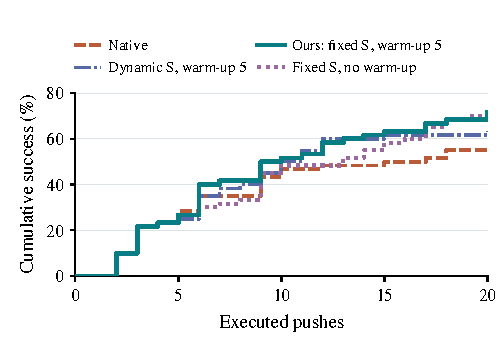
\includegraphics[width=\columnwidth]{figures/figS_rope_success_budget.pdf}
\captionof{figure}{\textbf{Rope success versus push budget.} Cumulative success over the same targets and three seeds as \cref{tab:rope-ablation}. Fixed memory with warm-up reaches the most goals within the budget.}
\label{fig:rope-budget}
\par}
\par\smallskip
Fixed memory with warm-up gives the best CD, success, and push count among the matched three-push variants. Anchoring memory at the stall lowers CD in every seed relative to earlier frames, supporting correction at the observed stalled region. More runs reach the goal within the same budget.\par

\par\smallskip
The terminal-frame objective scales memory by goal distance without horizon averaging. Stored stall observations persist across plans, so the correction continues to discourage returns to the same configuration.
\end{minipage}\par

\end{table*}
\clearpage
\begin{table*}[!t]
\par\smallskip
\noindent \begin{minipage}[t]{\columnwidth}
\vspace{0pt}
\section{Simulator rollouts}
\label{sec:renderings}
The visualizations connect the aggregate gains to changes in execution. Rope, PushT, and Maze detour examples use recorded frames; the remaining path panels render logged Pymunk and MuJoCo states. Starts and goals are shared within each pair.
\end{minipage}\hfill
\begin{minipage}[t]{\columnwidth}
\vspace{0pt}
\Cref{fig:rope-rollouts} aligns independently executed runs by push count. This exposes how the rope approaches its target shape under the same action budget. ECP reaches the goal in (a); in (b), its final shape is closer to the target, as reflected by lower Chamfer distance.
\end{minipage}\par
\par\smallskip
{\centering
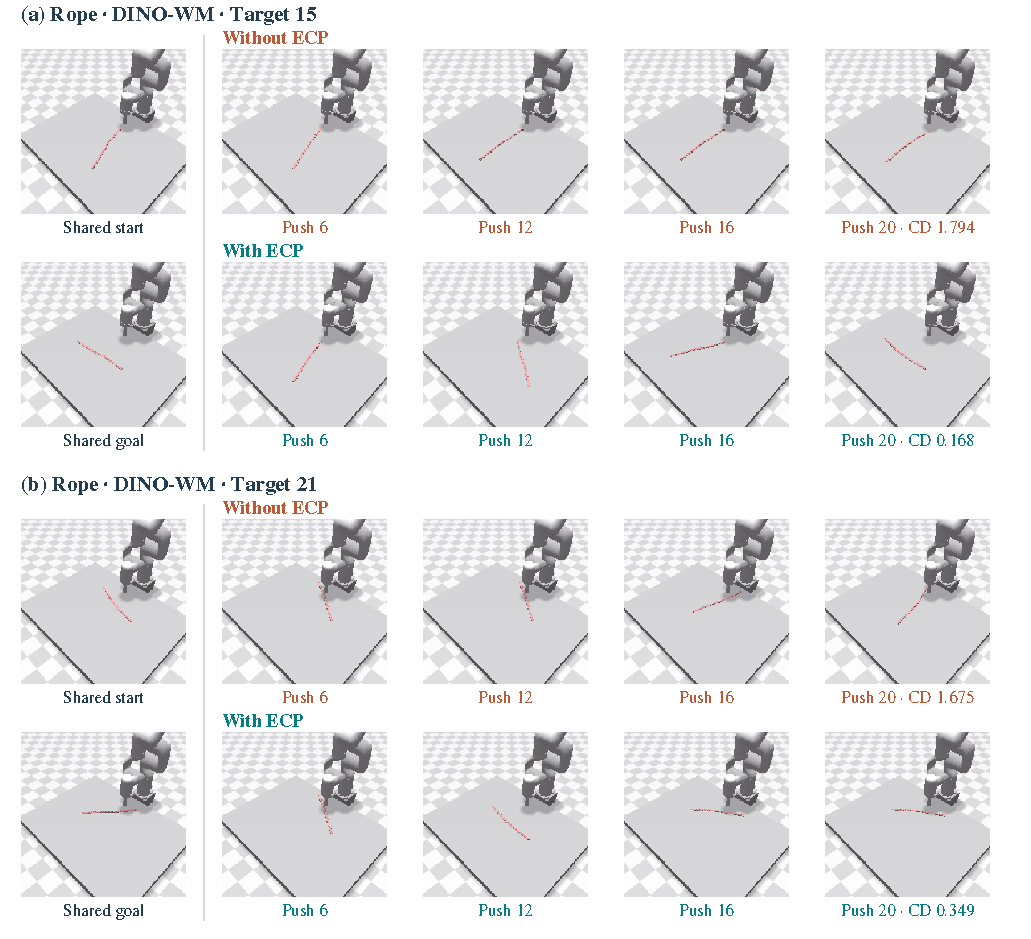
\includegraphics[width=\textwidth]{figures/figS_rope_rollouts.pdf}
\captionof{figure}{\textbf{Rope trajectories at equal push counts.} Brown/teal denote native planning/fixed-strength ECP with five warm-up pushes, using the same fixed DINO-WM, start, and goal. Columns align executed pushes. CD is final Chamfer distance (lower is better; success $<0.3$). ECP succeeds in (a); in (b), it lowers CD but both runs fail.}
\label{fig:rope-rollouts}
\par}
\par\smallskip
\noindent \begin{minipage}[t]{\columnwidth}
\vspace{0pt}
Rope requires coordinated pushes to change shape. Per-push observation retains execution feedback within each action block. The matched frames show the resulting geometry under a shared push budget.
\end{minipage}\hfill
\begin{minipage}[t]{\columnwidth}
\vspace{0pt}
In \cref{fig:rope-cd}, terminal CD is carried forward after success; shading shows variation across seed means. \Cref{fig:rope-budget} tracks completed targets, complementing geometric progress with completion speed.
\end{minipage}\par

\end{table*}
\clearpage
\begin{table*}[!t]
\par\smallskip
\noindent \begin{minipage}[t]{\columnwidth}
\vspace{0pt}
\Cref{fig:diverse-execution} compares recovery across object geometries and maze layouts. Shared starts and goals make the change in execution directly visible. Native planning repeats local motion; ECP changes the route under fixed or online-adapted world models.
\end{minipage}\hfill
\begin{minipage}[t]{\columnwidth}
\vspace{0pt}
Changing the approach to an object can complete alignment; leaving a revisited corridor can open a route to the goal. Both behaviors use the recent stall to condition the next planning objective.
\end{minipage}\par
\par\smallskip
{\centering
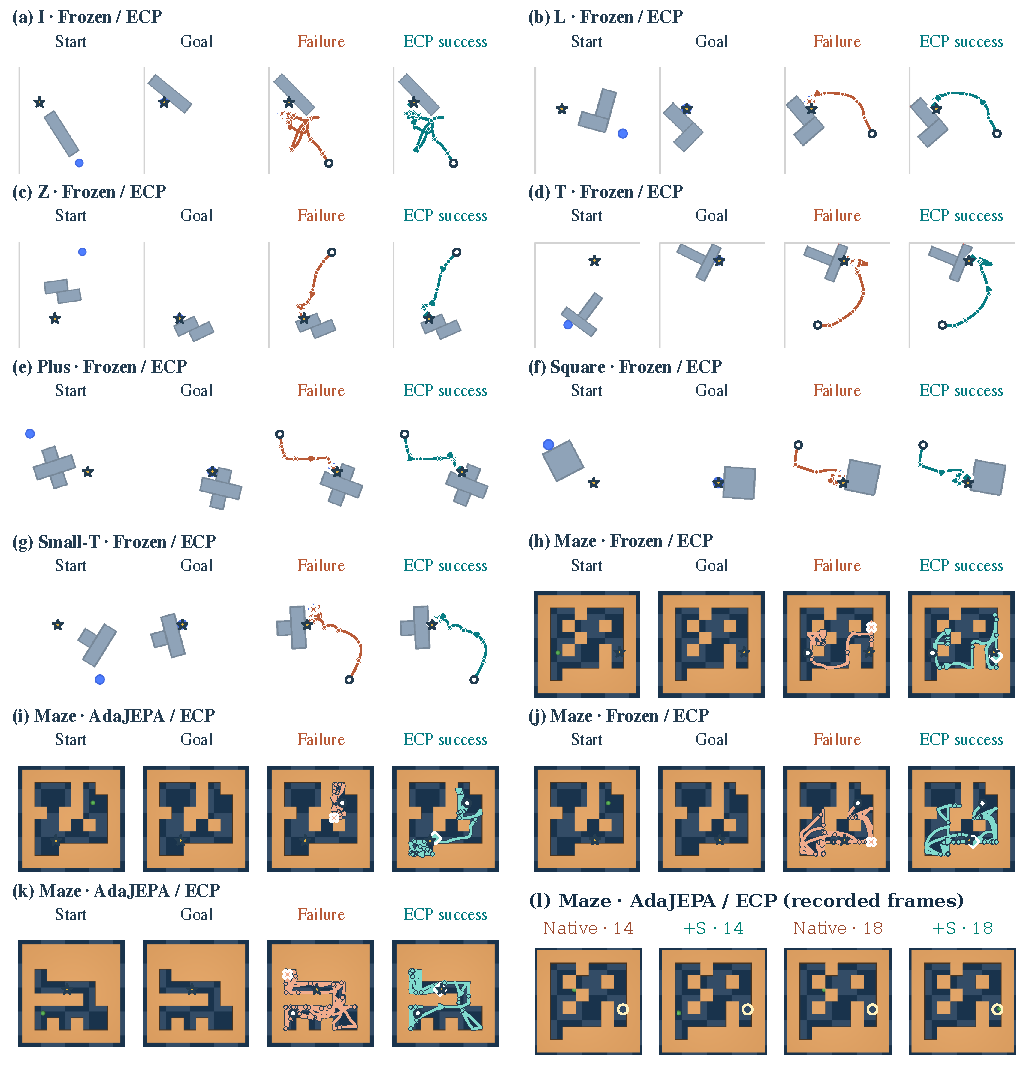
\includegraphics[width=\textwidth]{figures/figS_diverse_execution_maze.pdf}
\captionof{figure}{\textbf{ECP recovers stalls across seven PushObj shapes and three Maze tasks.} Brown and teal paths trace planning without and with ECP from the same start (circle) to their endpoints (cross or diamond). Stars mark goals and dots mark five-control blocks. Frozen fixes the pretrained ResNet, while AdaJEPA updates it online.}
\label{fig:diverse-execution}
\par}
\par\smallskip
\noindent \begin{minipage}[t]{\columnwidth}
\vspace{0pt}
The examples retain all seven PushObj shapes and three distinct Maze cases. In manipulation, changing the approach to the object completes alignment; in navigation, leaving a revisited corridor opens a route to the goal. Both use the recent stall to condition subsequent planning.
\end{minipage}\hfill
\begin{minipage}[t]{\columnwidth}
\vspace{0pt}
\section{Limitations and future directions}
\label{sec:pending}
ECP uses the current representation to identify revisited states. Shift-invariant stall features would extend this mechanism to stronger appearance changes. Source-disjoint tasks and held-out training seeds provide a next test of transfer~\cite{henderson2018matters,agarwal2021statistical}. Recovery trajectories also offer supervision for chunked policies~\cite{zhao2023act}, allowing successful corrections to be reused across episodes.
\end{minipage}\par

\end{table*}
\clearpage
\begin{table*}[!t]
\par\smallskip
\noindent \begin{minipage}[t]{\columnwidth}
\vspace{0pt}
\paragraph{Recovery under visual shifts.}
The PushT pairs in \cref{fig:pusht-rollouts} hold the LeWM weights, task, and execution budget fixed while switching ECP on or off. The red-agent case changes the pusher's appearance; the red-goal case changes the target cue. These examples test whether execution feedback can recover a stalled plan under two distinct visual changes.
\end{minipage}\hfill
\begin{minipage}[t]{\columnwidth}
\vspace{0pt}
ECP completes both tasks while native planning repeats local motion until the control limit. The snapshots show the intervening physical interaction and final alignment, complementing the aggregate visual-shift results. Each sequence ends at its actual stopping point, and the rightmost image gives the common goal observation.
\end{minipage}\par
\par\smallskip
{\centering
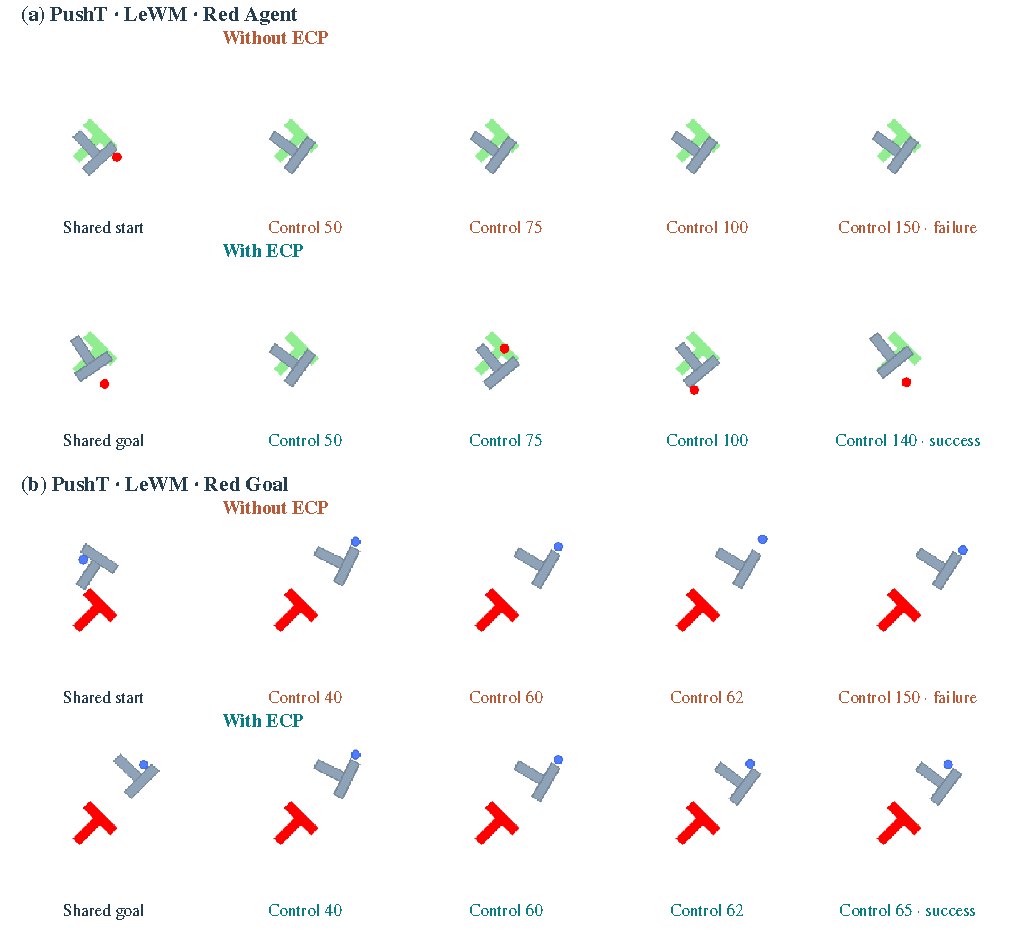
\includegraphics[width=\textwidth]{figures/figS_pusht_rollouts.pdf}
\captionof{figure}{\textbf{ECP recovers PushT under color shifts.} Paired runs use the same fixed LeWM, start, goal, and 150-control budget. Brown/teal label planning without/with ECP; frame numbers count executed controls. ECP succeeds under both red-agent and red-goal shifts, while native planning exhausts its budget. The right column shows the goal observation.}
\label{fig:pusht-rollouts}
\par}

\end{table*}
\clearpage
\begin{table*}[!t]
\par\smallskip
\noindent \begin{minipage}[t]{\columnwidth}
\vspace{0pt}
\paragraph{Navigation requires useful detours.}
\Cref{fig:maze-detour} examines why a temporary increase in goal distance can be productive. In the adaptive-model example, ECP leaves a repeatedly visited corridor, rounds the wall, and reaches the goal. The distance trace and recorded frames identify the detour and its subsequent progress.
\end{minipage}\hfill
\begin{minipage}[t]{\columnwidth}
\vspace{0pt}
The frozen-model example shows the same recovery pattern without changing world-model weights. It directly illustrates how execution-conditioned memory changes planning. Control indices expose motion within a planning block; five controls correspond to one step. The paths and distance traces use the actual executed trajectories.
\end{minipage}\par
\par\smallskip
{\centering
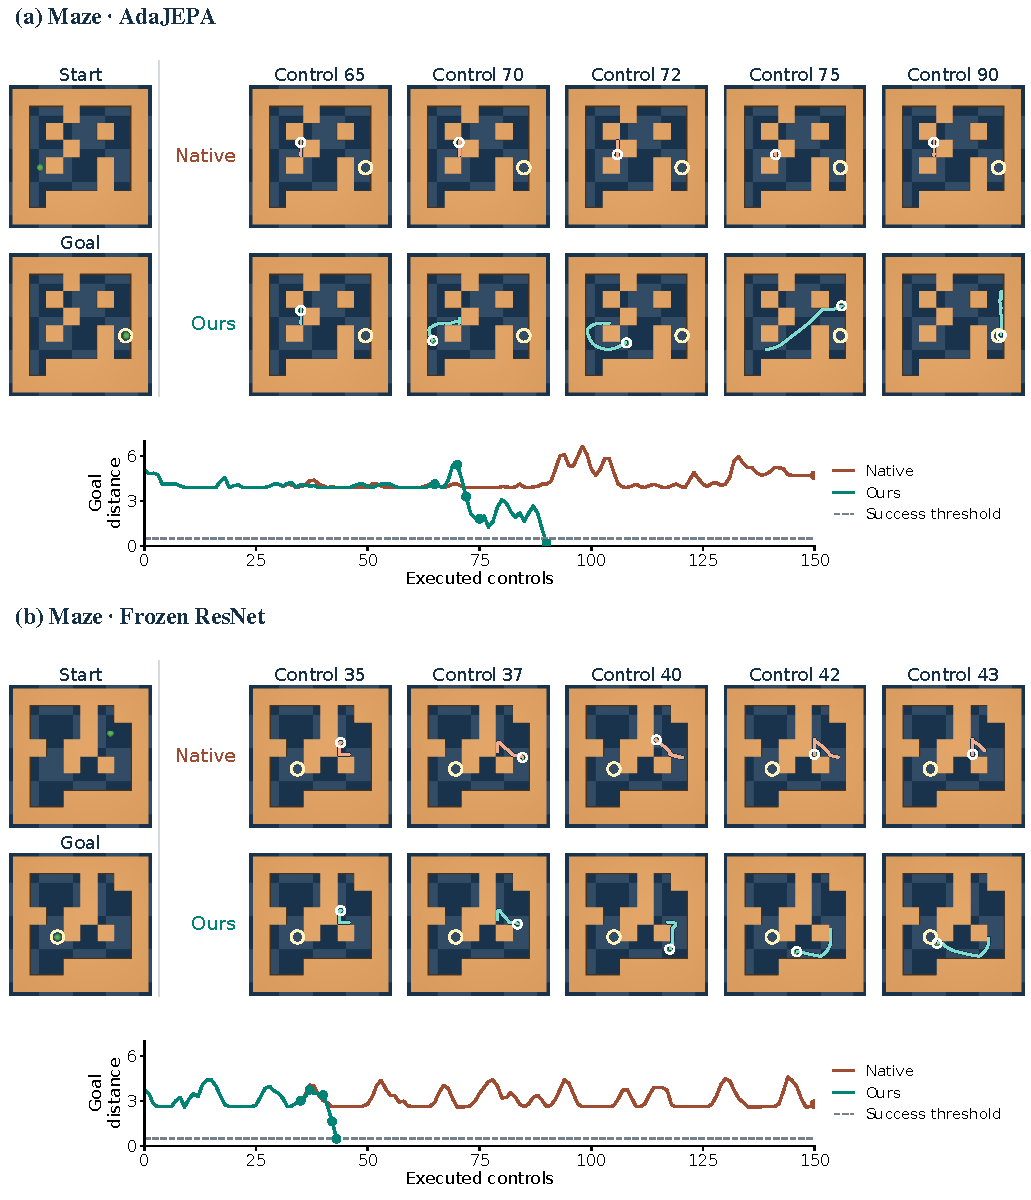
\includegraphics[width=\textwidth]{figures/figS_maze_detour_rollout.pdf}
\captionof{figure}{\textbf{Maze recoveries with adaptive and frozen ResNet world models.} Each row shows five recorded frames from one run. Columns align the two planners by executed control. Trails cover the preceding four controls, the white ring marks the agent, and the pale ring marks the goal. In (a), Ours briefly moves farther away to round a wall and reaches the goal at control 90. In (b), Ours reaches the goal at control 43 with the pretrained ResNet held fixed. Both native runs exhaust the 150-control budget.}
\label{fig:maze-detour}
\par}

\end{table*}
